\documentclass[11pt]{article}
\usepackage[pdftex]{graphicx}
\usepackage{amsmath, amsthm, amssymb, amsfonts, mathtools, graphicx, enumerate}
\usepackage{times}
\usepackage{booktabs}
\usepackage{url}
\usepackage{color,soul}
\usepackage{enumerate}
\usepackage{listings}
%%\usepackage{enumitem}
\newcommand{\R}{\mathbb{R}}
\setlength{\parindent}{0pt}
\setlength{\parskip}{1ex}
\setlength{\oddsidemargin}{0.0in}
\setlength{\textwidth}{6.5in}
\setlength{\topmargin}{-0.5in}
\setlength{\textheight}{9.0in}
\newcommand{\RR}{\mathbb{R}}
\newcommand{\labelsymbol}{t}
\newcommand{\answer}[1]{{\mbox{}\color{red}{#1}}}
\newcommand{\emptycheck}{\text{(\hspace{-.75ex}(\hspace{3ex})\hspace{-.75ex})}}
\newcommand{\checkans}[1]{\text{(\hspace{-.75ex}(\hspace{1ex}{#1}\hspace{1ex})\hspace{-.75ex})}}
\newcommand{\argmax}{{\mbox{arg}\hspace{-.1ex}}\max}
\usepackage{hyperref}
\DeclarePairedDelimiter{\norm}{\lVert}{\rVert}
\title{EECS 498: Reinforcement Learning \protect \\ Homework 4 Responses}
\author{Tejas Jha \\ tjha}
\usepackage{amsmath}
\usepackage{verbatim}
\usepackage{enumitem}

\begin{document}

\maketitle
This document includes my responses to Homework 4 questions. Responses that involved the use of coding will provide references to specific lines of code to provide a better overview of how the problem was approached. The code can either be referenced in the Appendix or in the accompanied python script submitted with this assignment.

\section*{Question 1}
\begin{enumerate}[label=(\alph*)]
\item
In this specific problem, we are able to set epsilon to 0 because we begin with optimistic initial values. We covered optimistic initial values in the bandit setting, but similarly in this specific problem, these values will encourage initial exploration until values are brought down to a point where the estimated values approach the expected values for the greedy actions.

\item
Below is a generated plot similar to the left part of Figure 12.10 from the textbook for the requested trace and alpha values using replacing traces.

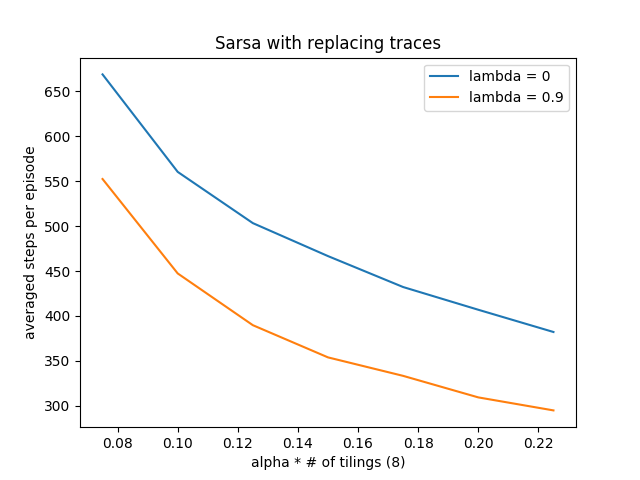
\includegraphics[scale=0.8]{replacing_traces.png}

\item
Below is a generated plot similar to the left part of Figure 12.10 from the textbook for the requested trace and alpha values using accumulating traces.

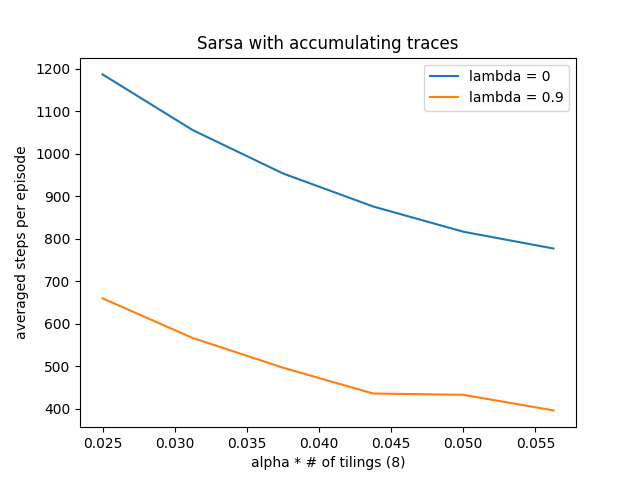
\includegraphics[scale=0.8]{accumulating_traces.png}

\item
If we change the range of the alphas to be same as that which we used to generate the plot in part (b) for accumulating traces, we can expect a plot with lower average steps than the plot in part (c) where accumulating traces was also used. This will be due to the larger alpha values being looked at which will now focus at the points on the curve that are lower. However, if we were to compare the plot in part (b) that used replacing traces , we will see that the curve for 0 lambda would be the same but the curve for 0.9 lambda would be lower for the accumulating traces. This result would suggest that using accumulating traces for this range of alphas seems to perform better as the averaged step per episode is lower, indicating a more optimal policy. While some searching online seems to indicate that replacing traces generally perform better than accmulating traces (http://www.incompleteideas.net/book/ebook/node80.html) as accumulating traces could end up selecting the "wrong" action more times resulting in a larger trace corresponding to the "wrong" action. As a result of this, accumulating traces generally take longer to learn to account for the larger trace for the "wrong" action. However, from the given alpha values, accumulating traces seems to work better in this situation, indicating that the optimal action could have been chosen earlier and then greedily selected more often with accumulating traces.

\end{enumerate}

\section*{Question 2}
Below are the reproduced Figures 13.1 and 13.2 from the textbook. The corresponding code used to genereate these igures can be found in the appendix. 

For fig1: Note that the blue curve is for $2^{-12}$, the orange curve is for $2^{-13}$ and the green curve is for $2^{-14}$. Also the data has been averaged over 100 trials.

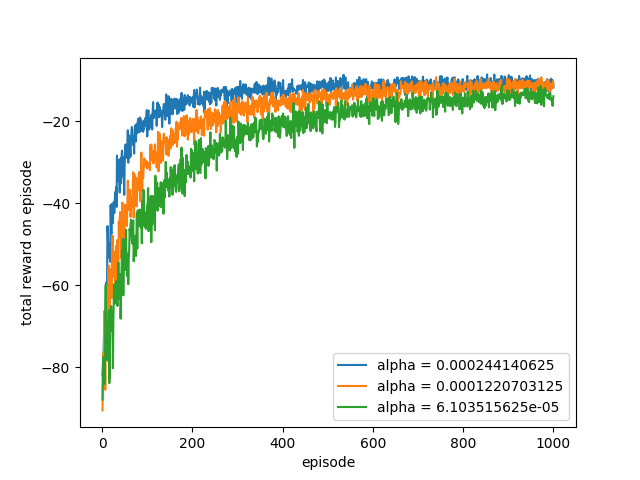
\includegraphics[scale=0.8]{fig1.png}

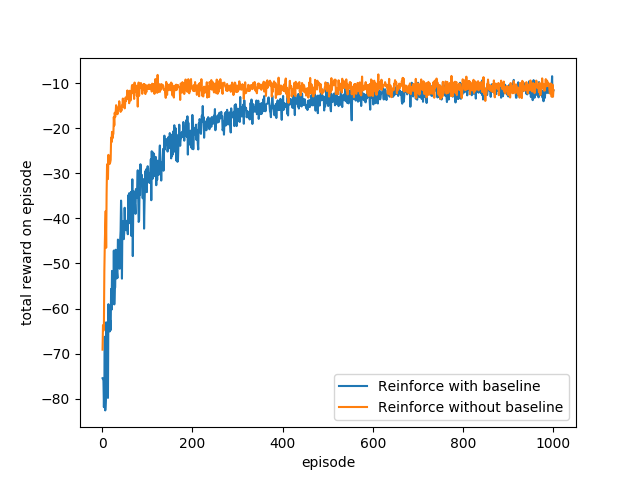
\includegraphics[scale=0.8]{fig2.png}

\section*{Question 3}
Below are the attempts made to recreate Figures 4 and 5 from the Options paper. The corresponding code used to genereate the plots for these figures can be found in the appendix.

\section*{Appendix: Relevant Code - tjha\_hw4.py}
\lstinputlisting[language=Python, breaklines=true, numbers=left]{tjha_hw4.py}   
\end{document}
